\section{Integrais duplas em coordenadas polares}
\label{sec:int2polar}

Tendo como base o conhecimento acumulado nas seções anteriores, agora
é possível expandir o problema do cálculo de área em coordenadas
polares para o problema do volume em coordenadas polares.

Revisitando o problema do cálculo do volume do sólido limitado abaixo
pelo plano $z = 0$ e acima pelo parabolóide $z = 1 - x^2 - y^2$ (ver
figura~\ref{fig:voldif} na página~\pageref{fig:voldif}),
utilizaremos um artifício para dividir a
base do sólido (o disco $D$) em diversos \emph{retângulos polares} e, a
partir desses retângulos, faremos o cálculo do volume.

Um \textbf{retângulo polar} (figura~\ref{fig:retangpolar}) é a região
formada pelo conjunto de coordenadas polares delimitadas por dois
ângulos e duas distâncias:

\begin{equation}
R = \{(r,\theta)\, | \, a \le r \le b,
\alpha \le \theta \le \beta\}
\end{equation}

\begin{figure}[H]
  \begin{center}
    \caption{O retângulo polar}
    \label{fig:retangpolar}
    \fbox{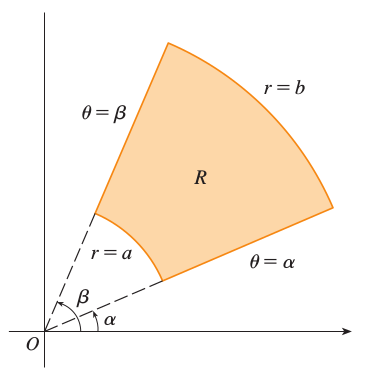
\includegraphics[scale=0.45]{imagens/int29.png}}\\
    \footnotesize{James Stewart: \emph{Cálculo} (8ª ed.,\ vol.\ 2, pg.\ 904)}
  \end{center}
\end{figure}

Usando o conceito de retângulos polares, dividimos a base do sólido (o
disco $D$ na figura~\ref{fig:voldif}) em vários retângulos polares,
conforme ilustrado na figura~\ref{fig:retangpolar2} a seguir, com as
seguintes características:

\begin{itemize}
  \item O intervalo $[a, b]$ é dividido em $m$ intervalos $[r_{i-1},
    r_i]$, de larguras \emph{iguais}:
    \begin{equation*}
      \Delta r = \frac{b-a}{m}
    \end{equation*}
  \item O intervalo $[\alpha, \beta]$ é dividido em $n$ intervalos
    $[\theta_{j-1}, \theta_j]$, de larguras \emph{iguais}:
    \begin{equation*}
      \Delta \theta = \frac{\beta - \alpha}{n}
    \end{equation*}
  \item O centro de cada retângulo polar é dado por:
    \begin{equation*}
      r_i^* = \frac{1}{2}(r_{i-1}+r_i) \quad\ \quad\ \text{ e }
      \quad\ \quad\ \theta_j^* = \frac{1}{2}(\theta_{j-1}+\theta_j)
    \end{equation*}
\end{itemize}

\begin{figure}[H]
  \begin{center}
    \caption{Divisão da base do sólido em retângulos polares}
    \label{fig:retangpolar2}
    \fbox{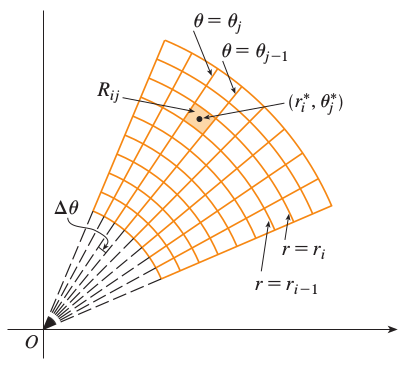
\includegraphics[scale=0.45]{imagens/int30.png}}\\
    \footnotesize{James Stewart: \emph{Cálculo}\\ (8ª ed.,\ vol.\ 2, pg.\ 904)}
  \end{center}
\end{figure}

Podemos então calcular a área de \emph{cada retângulo polar} usando a
equação~\ref{eq:areasetor} da seguinte maneira:

\begin{equation}
  \label{eq:arearetangpolar}
  \begin{split}
    \Delta A_i &= \left(\frac{1}{2} r_i^2\Delta \theta\right) - \left(\frac{1}{2} r_{i-1}^2\Delta \theta\right)\\
               &= \frac{1}{2}(r_i^2 - r_{i-1}^2)\Delta \theta\\
               &= \ldots\\
               &= \color{red}r_i^*\color{black} \Delta r \Delta \theta
  \end{split}
\end{equation}

Note que na equação~\ref{eq:arearetangpolar}, que calcula a área de
cada retângulo polar, surgiu um fator $r_i^*$ que multiplica $\Delta r
\Delta \theta$. Esse fator é necessário para levar em conta que
retângulos mais distantes da origem terão área maior (do contrário,
como dividimos os setores em larguras iguais, todos os retângulos
teriam a mesma área, o que não faz sentido\footnote{Um vídeo
  disponível em uma página da Universidade do Texas fornece uma
  explicação interessante para isso:
  \url{https://web.ma.utexas.edu/users/m408m/Display15-4-2.shtml}}).

Agora que já sabemos como calcular a área de cada retângulo polar da
base de nosso sólido, vamos expandir o raciocínio para o volume do
prisma que tem como base o retângulo polar e altura até a superfície
da função, conforme ilustrado na figura~\ref{fig:prismapolar} a
seguir:

\begin{figure}[H]
  \begin{center}
    \caption{Volume do sólido que tem como base o retângulo polar}
    \label{fig:prismapolar}
    \fbox{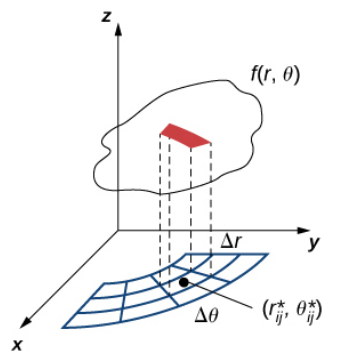
\includegraphics[scale=0.5]{imagens/int31.png}}\\
    \footnotesize{Gilbert~Strang~\&~Edwin~ Herman:\\ \emph{Calculus}
        (ed.\ online, 2017, vol.\ 3, pg.\ 527)}
  \end{center}
\end{figure}

O volume de cada prisma será dado pela multiplicação da área de sua base,
$\Delta A_i$, com sua altura, dada em coordenadas polares por $f[r_i^*
  \cos(\theta_j^*), r_i^* \sin(\theta_j^*)]$:

\begin{equation}
      V_{R_{ij}} \approx f[r_i^* \cos(\theta_j^*), r_i^* \sin(\theta_j^*)] \Delta A_i
\end{equation}

E a estimativa do volume total sob o sólido é dada pela somatória do
volume individual de todos os prismas:

\begin{equation}
  \begin{split}
    V &\approx \sum_{i=1}^m \sum_{j=1}^n f[r_i^* \cos(\theta_j^*),
    r_i^* \sin(\theta_j^*)] \Delta A_i\\
      &\approx \sum_{i=1}^m \sum_{j=1}^n f[r_i^* \cos(\theta_j^*),
    r_i^* \sin(\theta_j^*)] \color{red}r_i^*\color{black}\Delta r
    \Delta \theta
  \end{split}
\end{equation}

Perceba que à medida em que aumentamos o número de prismas (à medida
em que os retângulos polares ficam menores), a estimativa do cálculo
do volume fica mais precisa. No limite, quando o número de retângulos
polares tendo ao infinito, o volume tende ao valor exato, e essa é a
idéia de usar coordenadas polares para o cálculo de volumes:

\begin{equation}
  \begin{split}
    V &= \lim_{m,n \to \infty} \sum_{i=1}^m \sum_{j=1}^n f[r_i^* \cos(\theta_j^*),
      r_i^* \sin(\theta_j^*)] \Delta A_i\\
      &= \iint\displaylimits_R f[r \cos(\theta), r \sin(\theta)]
    \diff A\\
      &= \int_\alpha^\beta \int_a^b f[r \cos(\theta), r
      \sin(\theta)] \color{red}r\color{black} \diff r \diff \theta
  \end{split}
\end{equation}

Em resumo, quando temos uma função de difícil integração quando
expressa em coordenadas retangulares, $\displaystyle \int_a^b \int_c^d f(x, y) \diff
y \diff x$,
podemos reexpressar a mesma função em coordenadas polares,
$\displaystyle \int_\alpha^\beta \int_a^b f[r \cos(\theta), r
      \sin(\theta)] r \diff r \diff \theta$,
para facilitar o cálculo.
